\textbf{Q1. Search: Algorithms}

\begin{tabular}{l@{\hspace{0.15\linewidth}}c}
\begin{minipage}{0.45\linewidth}

Consider the state space search problem shown to the right.
$A$ is the start state and the shaded states are goals.
Arrows encode possible state transitions, and numbers by the arrows represent action costs.
Note that state transitions are directed; for example, $A \rightarrow B$ is a valid transition, but $B \rightarrow A$ is not.
Numbers shown in diamonds are heuristic values that estimate the optimal (minimal) cost from that node to a goal.

\end{minipage}

&

\begin{minipage}{0.34\linewidth}

  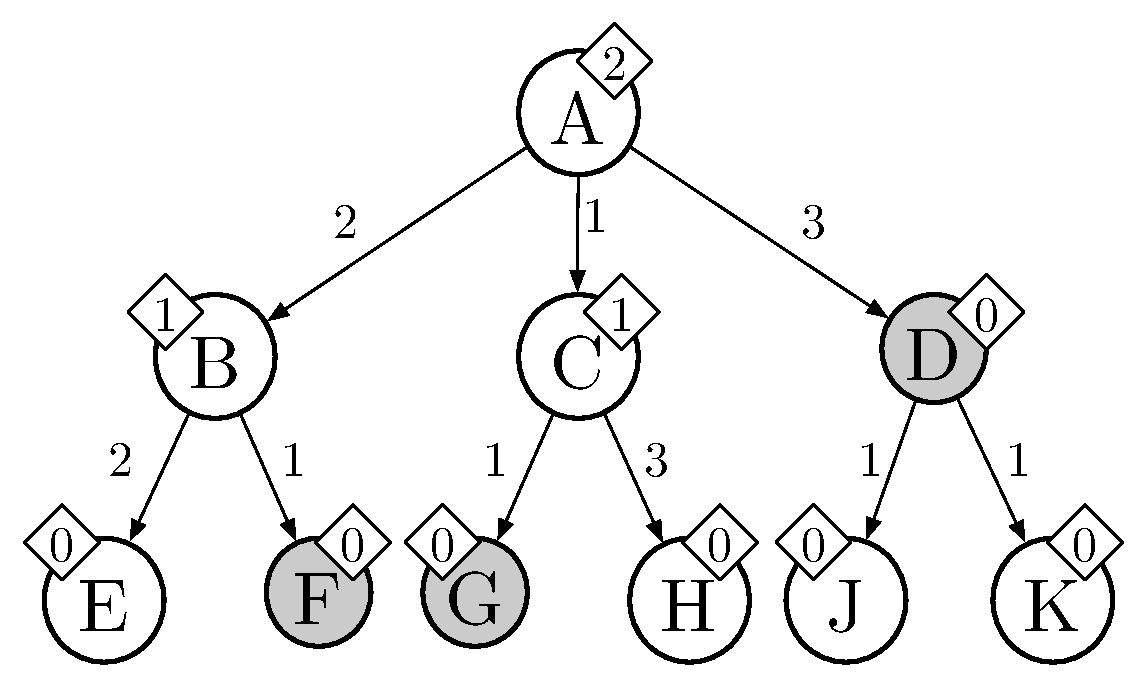
\includegraphics[height=1.6in]{figures/search_tree.pdf}

\end{minipage}

\end{tabular}


For each of the following search algorithms, write down the nodes that are removed from fringe in the course of the search, as well as the final path returned.
Because the original problem graph is a tree, the tree and graph versions of these algorithms will do the same thing, and you can use either version of the algorithms to compute your answer.

Assume that the data structure implementations and successor state orderings are all such that \emph{ties are broken alphabetically}.
For example, a partial plan $S \rightarrow X \rightarrow A$ would be expanded before $S \rightarrow X \rightarrow B$; similarly, $S \rightarrow A \rightarrow Z$ would be expanded before $S \rightarrow B \rightarrow A$.

\vfill

\begin{enumerate}
\item {\bf Depth-First Search (ignores costs) [5 pts]}
\vfill
  \textbf{Nodes removed from fringe:} {\color{red} A, B, E, F} \\
  \textbf{Path returned:} {\color{red} A, B, F} \\
\item {\bf Breadth-First Search (ignores costs) [5 pts]}
\vfill
  \textbf{Nodes removed from fringe: } {\color{red}  A, B, C, D}\\
  \textbf{Path returned: }  {\color{red} A, D}\\
\item {\bf Uniform-Cost Search [5 pts]}
\vfill
  \textbf{Nodes removed from fringe: } {\color{red} A, C, B, G}\\
  \textbf{Path returned: }  {\color{red}  A, C, G}\\
\item {\bf Greedy Search [5 pts]} 
\vfill
  \textbf{Nodes removed from fringe: } {\color{red}  A, D}\\
  \textbf{Path returned: }  {\color{red}  A, D}\\
\item {\bf A* Search [5 pts]} \\
  \textbf{Nodes removed from fringe: } {\color{red} A, C, G}\\
  \textbf{Path returned: } {\color{red} A, C, G} \\
\end{enumerate}	



\newpage

\textbf{Q2. Search: Heuristic Function Properties} \\

For the following questions, consider the search problem shown on the left.
It has only three states, and three directed edges.
$A$ is the start node and $G$ is the goal node.
To the right, four different heuristic functions are defined, numbered I through IV.

\begin{tabular}{c@{\hspace{0.1\linewidth}}c}

\begin{minipage}{0.45\linewidth}

\centering
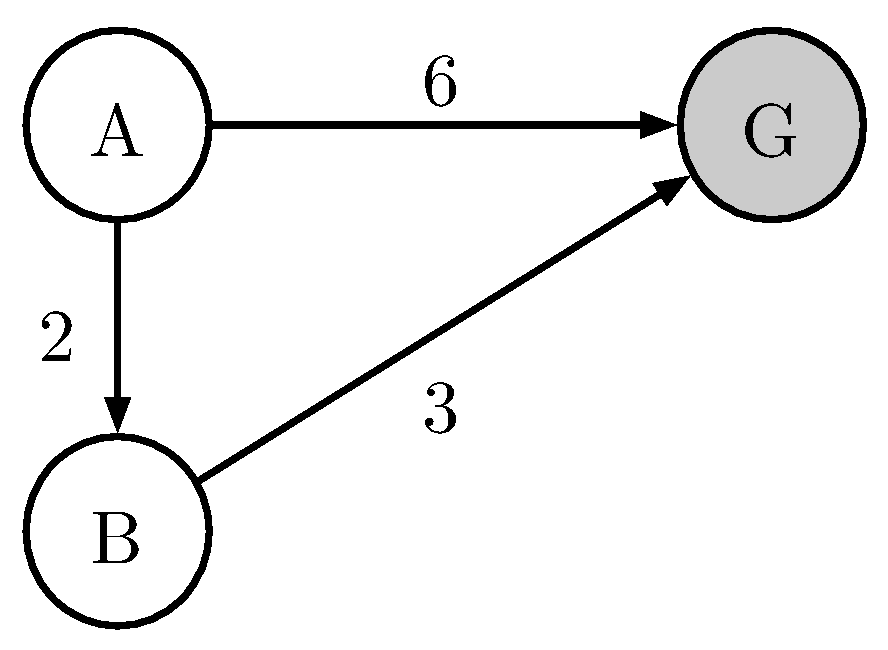
\includegraphics[height=1.4in]{figures/heuristic_triangle.pdf}

\end{minipage}

&

\begin{minipage}{0.45\linewidth}

  {\large
  \begin{tabular}{|l|ccc|}
      \hline
      & h($A$) & h($B$) & h($G$) \\ \hline
  I   & 4    & 1 & 0    \\ \hline
  II  & 5    & 4 & 0    \\ \hline
  III & 4    & 3 & 0    \\ \hline
  IV  & 5    & 2 & 0    \\ \hline
  \end{tabular}
  }

\end{minipage}
\end{tabular}


\paragraph*{\bf Admissibility and Consistency}

For each heuristic function, circle whether it is admissible and whether it is consistent with respect to the search problem given above.

\vspace{.5cm}
\begin{table}[!h]
\caption{}
\centering
\begin{tabular}{|m{0.8in}|m{0.8in} m{0in}|m{0.8in} m{0in}|}
   \hline
   ~   & Admissible?                     & ~ & Consistent?                     & ~ \\ [0.15in] \hline
   I [5 pts]  & {\color{red} Yes} \hfill No  & ~ & Yes \hfill {\color{red} No}  & ~ \\ [0.15in] \hline
   II [5 pts] & Yes \hfill {\color{red} No}  & ~ & Yes \hfill {\color{red} No}  & ~ \\ [0.15in] \hline
   III [5 pts] & {\color{red} Yes} \hfill No  & ~ & {\color{red} Yes} \hfill No  & ~ \\ [0.15in] \hline
   IV [5 pts] & {\color{red} Yes} \hfill No  & ~ & Yes \hfill {\color{red} No}  & ~ \\ [0.15in] \hline
\end{tabular}
\end{table}